\documentclass[11pt,a4paper]{article}
\usepackage[margin=2.4cm]{geometry}
\usepackage{amsmath,amssymb,booktabs,hyperref,graphicx}
\newcommand{\dtau}{\Delta\tau}
\newcommand{\dt}{\Delta t}
\newcommand{\code}[1]{\texttt{\small #1}}
\newcommand{\tv}{\vartheta}   % all thermodynamic variables
\newcommand{\pv}{\varpi}      % pressure variable (pi or p)
\title{Moist split-explicit integration with a Verlet fast step:\\
vertically implicit acoustics and gravity, the pressure as an additional variable,\\
and a choice of the thermodynamic variable}
\author{MultiRate.jl}
\date{\today}
\emergencystretch=3em
\begin{document}
\maketitle

\begin{abstract}
This note puts together the moist model of \code{docs/exner} and the fast integrator of
\code{docs/verlet\_ei}. The state is $(\rho,U,W,X,\rho q_v,\rho q_c,\pv)$: density, momenta, one
thermodynamic variable $X$, two moisture densities, and the pressure ($\pv=p$) or the Exner pressure
($\pv=\pi$) as an additional prognostic variable. Because the momentum equations see only $\pv$ and
$\rho$, the fast acoustic--gravity system and its column solve do not depend on the choice of $X$.
Two choices are implemented and compared: the density potential temperature $X=\rho\theta_\rho$ and
the internal energy $X=\rho e$. The fast part is integrated with the Verlet step EI: horizontal
pressure force and horizontal divergence explicit, vertical acoustics and gravity implicit in one
tridiagonal system per column. The slow integrators are MIS, ETD (exponential Runge--Kutta) and
Lawson methods on the same frozen split. The transport of the two moisture variables is described
in detail (Section~\ref{sec:moisture}). Examples: the moist bubble of Bryan and Fritsch and the
moist flow over an Agnesi hill.
\end{abstract}

\tableofcontents

%======================================================================
\section{Equations}\label{sec:eq}
\subsection{Variables}
\begin{center}\small
\begin{tabular}{lll}\toprule
symbol & meaning & code\\\midrule
$\rho$ & total density (dry air, vapour, cloud water) & \code{irho}\\
$U=\rho u$, $W=\rho w$ & momenta at the $x$- and $z$-faces (C-grid) & \code{iU}, \code{iW}\\
$X$ & thermodynamic variable: $\rho\theta_\rho$ or $\rho e$ & \code{iTheta}\\
$V=\rho_v=\rho q_v$ & vapour density & \code{iV}\\
$C=\rho_c=\rho q_c$ & cloud water density & \code{iC}\\
$\pv$ & pressure variable: $\pi=(p/p_0)^{\kappa_d}$ or $p$ & \code{ipi}\\\bottomrule
\end{tabular}
\end{center}
$\tv=(\rho,X,V,C,\pv)$ denotes all cell-centred (thermodynamic) variables, $M=(U,W)$ the momenta.
The dry air density is $\rho_d=\rho-V-C$; the total water $q_t=q_v+q_c$ is diagnostic.

\subsection{The system}
\begin{align}
\partial_t\rho+\nabla\cdot M&=0,\label{eq:rho}\\
\partial_tM+\nabla\cdot(M\otimes v)&=-\nabla p-\rho g\,k,\label{eq:mom}\\
\partial_tX+\mathcal T_X(M)&=Q_X\,S_c,\label{eq:X}\\
\partial_tV+\nabla\cdot(q_vM)&=-S_c,\label{eq:V}\\
\partial_tC+\nabla\cdot(q_cM)&=S_c,\label{eq:C}\\
\partial_t\pv+\mathcal T_\pv(M)&=Q_\pv\,S_c.\label{eq:pv}
\end{align}
$\mathcal T_X$ is the transport operator of the thermodynamic variable (Section~\ref{sec:thvar}),
$S_c$ the condensation rate, and \eqref{eq:pv} the pressure equation that follows from the equation
of state by the chain rule (Section~\ref{sec:pressure}). There is no background state and no
saturation adjustment.

\subsection{Thermodynamics and phase change}
With the density-weighted quantities
\[
R_m=R_d\rho_d+R_v\rho_v,\qquad c_{pm}=c_{pd}\rho_d+c_{pv}\rho_v+c_{pl}\rho_c,\qquad c_{vm}=c_{pm}-R_m,
\]
the pressure is $p=R_mT$, the latent heat $L(T)=L_0+(c_{pv}-c_{pl})(T-T_0)$ (constants and $e_s(T)$
as in CGDycore). The temperature is an explicit function of $(\rho,X,V,C)$ for both choices of $X$.
Phase equilibrium is the complementarity condition
\[
\rho_c\ge0,\qquad\rho_{vs}(T)-\rho_v\ge0,\qquad\rho_c\,(\rho_{vs}(T)-\rho_v)=0,\qquad\rho_{vs}=\frac{e_s(T)}{R_vT},
\]
written with the Fischer--Burmeister function $\varphi_{FB}(a,b)=\tfrac12(a+b-\sqrt{a^2+b^2})$ as
$\varphi_{FB}(\rho_{vs}-\rho_v,\rho_c)=0$. The condensation rate is an explicit relaxation,
\[
S_c=-\frac{\varphi_{FB}\big(\rho_{vs}(T)-\rho_v,\ \rho_c\big)}{\tau},\qquad\tau=\tau_{\rm fac}\,\dtau_{\rm ac},
\]
with $\dtau_{\rm ac}=0.85\cdot0.92\,\Delta x/c_s$ the acoustic small step and $\tau_{\rm fac}=0.25$ by
default in the code; with the Verlet EI small step $\tau_{\rm fac}\ge0.5$ is needed (Section~\ref{sec:bubble}). $S_c$ is evaluated from the fast state in every small
step (\code{micro = :fast}). The phase change is isochoric and conserves the internal energy:
\[
\frac{\mathrm dT}{\mathrm d\rho_c}\Big|_{\rho,\,\rho e}=\frac{L-R_vT}{c_{vm}} .
\]

%======================================================================
\section{The pressure as an additional variable}\label{sec:pressure}
The momentum equation needs the pressure gradient only. With the Exner pressure of the \emph{dry}
exponent $\kappa_d=R_d/c_{pd}$ it is the exact product
\[
\nabla p=c_{pd}\,\hat\Theta\,\nabla\pi,\qquad\hat\Theta=\frac p{R_d\pi},
\]
and with the pressure itself simply $\nabla p$. In both cases write
\[
\nabla p=P\,\nabla\pv,\qquad P=c_{pd}\hat\Theta\ (\pv=\pi),\qquad P=1\ (\pv=p).
\]
The pressure variable has its own evolution equation. For any thermodynamic variable $X$ the
equation of state is $\pv=\pv(\rho,X,V,C)$, hence
\begin{equation}
\partial_t\pv=a\,\partial_t\rho+b\,\partial_tX+c\,\partial_tV+d\,\partial_tC,\qquad
(a,b,c,d)=\frac{\partial\pv}{\partial(\rho,X,V,C)} .\label{eq:chain}
\end{equation}
Inserting \eqref{eq:rho}, \eqref{eq:X}--\eqref{eq:C} gives a transport part, which is linear in the
mass flux $M$, and a phase source:
\[
\mathcal T_\pv(M)=a\,\nabla\cdot M+b\,\mathcal T_X(M)+c\,\nabla\cdot(q_vM)+d\,\nabla\cdot(q_cM),
\]
\[
Q_p=\frac{R_m(L-R_vT)}{c_{vm}}-R_vT,\qquad Q_\pi=\kappa_d\,\frac\pi p\,Q_p .
\]
$Q_p$ (latent heating minus the loss of gas constant) is the same for every $X$; it equals
$b\,Q_X+d-c$ of the respective equation of state. In continuous time \eqref{eq:pv} keeps $\pv$ on the
equation of state. The time discretization does not, so $\pv$ is recomputed from $(\rho,X,V,C)$ after
every large step (\code{frozen\_step\_end!}), not at the stages. The relative drift before this
reset is reported with the examples.

\paragraph{Consequence for the fast system.} Momentum reacts to $\pv$ and $\rho$ only; $\pv$ and
$\rho$ react to the momentum only. $X$, $V$ and $C$ do not appear in the momentum rows: within a
stage they are \emph{slaved} to the mass flux. The acoustic--gravity system is closed in
$(\rho,\pv,U,W)$, and the choice of the thermodynamic variable changes two things only: the row of
$X$ itself and the coefficients $b\,\mathcal T_X$ of the pressure row.

%======================================================================
\section{Thermodynamic variables}\label{sec:thvar}
\begin{center}\small
\begin{tabular}{p{2.6cm}p{5.9cm}p{5.9cm}}\toprule
& $X=\rho\theta_\rho$ (\code{thvar = :thetarho}) & $X=\rho e$ (\code{thvar = :energy})\\\midrule
definition & $p=p_0\big(R_dX/p_0\big)^{1/(1-\kappa_M)}$, $\kappa_M=R_m/c_{pm}$ &
$X=c_{vm}T+e_{0v}\rho_v$, $e_{0v}=L_0-(c_{pv}-c_{pl})T_0$\\
temperature & $T=\big(R_dX/p_0^{\kappa_M}\big)^{1/(1-\kappa_M)}/R_m$ & $T=(X-e_{0v}\rho_v)/c_{vm}$\\
transport $\mathcal T_X(M)$ & $\nabla\cdot(\theta_\rho M)$ & $\nabla\cdot(eM)+p\,\nabla\cdot(M/\rho)$\\
phase source $Q_X$ & $-X\,P_{BF}$ (Bryan--Fritsch prefactor) & $0$\\
conserved & $\int X$ without phase change & $\int X$ only for $\nabla\cdot v=0$\\\bottomrule
\end{tabular}
\end{center}
\paragraph{Density potential temperature.} $\theta_\rho$ with the moist exponent $\kappa_M$ is a
material invariant without phase change, so $X$ is in flux form. The latent heating is the source
$Q_X=-X\,P_{BF}$,
\[
P_{BF}=-\frac L{c_{pm}T}-\ln\frac p{p_0}\,\frac{R_m}{c_{pm}}\Big(\frac{R_v}{R_m}+\frac{c_{pl}-c_{pv}}{c_{pm}}\Big)+\frac{R_v}{R_m},
\]
which is the isochoric first law expressed in $\theta_\rho$ (\code{docs/exner}).

\paragraph{Internal energy.} With $e_d=c_{vd}T$, $e_v=c_{vv}T+e_{0v}$, $e_l=c_{pl}T$ the latent heat is
$L=h_v-h_l=e_{0v}+(c_{pv}-c_{pl})T$, consistent with $L(T)$ above. The internal energy does not
change in an isochoric phase change: $Q_X=0$, the latent heat is contained in $e_{0v}\rho_v$, and the
temperature is a linear function of $X$. The price is the compression work $p\,\nabla\cdot v$, which
is not a flux divergence. It is written with the mass flux,
\[
\partial_tX+\nabla\cdot(e\,M)+p\,\nabla\cdot\Big(\frac M\rho\Big)=0,
\]
so that it is linear in $M$ like every other transport term.

\paragraph{One form for both.} At a face $f$ with the mass flux $F_f$ (normal momentum times face
area) and for the adjacent cell $c$ both transport operators are
\begin{equation}
\mathcal T_X(M)\big|_c=\frac1{|c|}\sum_{f\in\partial c}\pm\,\chi_{c,f}\,F_f,\qquad
\chi_{c,f}=\begin{cases}\theta_{\rho,f}&X=\rho\theta_\rho,\\[1mm] e_f+\dfrac{p_c}{\bar\rho_f}&X=\rho e,\end{cases}\label{eq:chi}
\end{equation}
with the upwind face value $\theta_{\rho,f}$ or $e_f$ (third order, as for $q_v$ and $q_c$), the
pressure $p_c$ of the cell (from the prognostic $\pv$) and the face mean $\bar\rho_f$ of the density.
For the energy the coefficient is a face enthalpy; it differs between the two cells of a face by
$(p_c-p_{c'})/\bar\rho_f$, which is the discrete $v\cdot\nabla p$. The pressure row has the same form
with
\begin{equation}
\kappa_{c,f}=a_c+b_c\,\chi_{c,f}+c_c\,q_{v,f}+d_c\,q_{c,f} .\label{eq:kappa}
\end{equation}
Other variables fit the same form as long as $\mathcal T_X$ is linear in $M$ with coefficients that
can be frozen; the total energy (kinetic energy in the equation of state) is not implemented.

%======================================================================
\section{Transport of the two moisture variables}\label{sec:moisture}
Vapour and cloud water are two prognostic densities $V=\rho q_v$ and $C=\rho q_c$, not a total water
and a diagnostic split. Their transport has five properties.

\paragraph{1. Flux form with the mass flux of the continuity equation.} On the C-grid, with the
mass fluxes $F^x_{i,k}=J_xU_{i,k}$ at the $x$-faces and $F^z_{i,k}=\Omega_{i,k}=W_{i,k}-z_x\bar U$ at the
$\eta$-faces ($J=1$, $\Omega=W$ on a flat grid),
\begin{align*}
J\,\partial_t\rho_{i,k}&=-\frac{F^x_{i+1,k}-F^x_{i,k}}{\Delta x}-\frac{F^z_{i,k+1}-F^z_{i,k}}{\Delta\eta},\\
J\,\partial_tV_{i,k}&=-\frac{q^x_{v,i+1,k}F^x_{i+1,k}-q^x_{v,i,k}F^x_{i,k}}{\Delta x}
-\frac{q^z_{v,i,k+1}F^z_{i,k+1}-q^z_{v,i,k}F^z_{i,k}}{\Delta\eta}-J\,S_{c,i,k},
\end{align*}
and the same for $C$ with $q_c$ and $+S_c$. The fluxes are those of $\rho$, multiplied by a face
value of the specific humidity.

\paragraph{2. Face values frozen, mass flux live.} The face values $q^x_v$, $q^z_v$, $q^x_c$, $q^z_c$
are third-order upwind reconstructions of the cell values $q_v=V/\rho$, $q_c=C/\rho$ of the stage
value $y$ (\code{aface\_x}, \code{aface\_z}; upwind with respect to the mass flux of $y$; the same
reconstruction as for $\theta_\rho$ or $e$). They are part of the coefficient vector $C(y)$ and
constant during the fast integration. The mass fluxes are those of the evolving fast state $z$.
The moisture transport is therefore entirely in the \emph{fast} part, bilinear in (frozen face
value)$\times$(live momentum):
\[
\partial_tV=-\nabla\cdot\big(q_{v,f}(y)\,M(z)\big)-S_c(z),\qquad\partial_tC=-\nabla\cdot\big(q_{c,f}(y)\,M(z)\big)+S_c(z).
\]
There is no moisture advection in the slow part; the slow part contains the momentum advection
only. For $z=y$ the sum is the full operator, $N(q)=F(q,q)$.

\paragraph{3. Updated with the same momenta as $\rho$, in every substep.} In the Verlet step
(Section~\ref{sec:ei}) $V$ and $C$ are thermodynamic rows like $\rho$: explicit in the horizontal
flux of the new $U$, and implicit in the vertical flux. They do not enter the column system; after
the tridiagonal solve for $W^{n+1}$ they follow by back substitution,
\[
V_k^{n+1}=R_{V,k}-\frac{\beta h}{\Delta z}\big(q^z_{v,k+1}W^{n+1}_{k+1}-q^z_{v,k}W^{n+1}_k\big),
\]
with the same $W^{n+1}$ as $\rho^{n+1}$ and $\pv^{n+1}$. Hence in every substep, and for every stage of
MIS, ETD and Lawson:
\begin{itemize}
\item \emph{consistency with the continuity equation}: for $q_v\equiv q$ constant in space all face
values equal $q$ and $\partial_tV=q\,\partial_t\rho$ exactly, also through the implicit vertical
step; a constant specific humidity stays constant;
\item \emph{conservation}: $\sum J\,(V+C)$ is conserved to round-off (the phase change moves water
between $V$ and $C$), and so are $\sum J\rho$ and $\sum J\rho_d$;
\item \emph{vertical Courant number}: the vertical moisture flux is implicit in $W$ with the frozen
face value, so thin layers do not restrict the small step through the acoustic part of the
moisture transport.
\end{itemize}

\paragraph{4. Moisture in the pressure equation.} The pressure equation contains
$c\,\partial_tV+d\,\partial_tC$ \eqref{eq:chain}: the moisture fluxes enter the coefficient
$\kappa_{c,f}$ \eqref{eq:kappa} with the same face values $q_{v,f}$, $q_{c,f}$. This is the only way
moisture feeds back on the dynamics during a stage (together with $\rho=\rho_d+V+C$ in gravity).

\paragraph{5. Phase change.} $\mp S_c$ is evaluated from the fast state in every small step, in the
explicit horizontal part of the step, together with $Q_XS_c$ in the $X$ row and $Q_\pv S_c$ in the
pressure row ($Q_X$, $Q_\pv$ frozen per cell). $\varphi_{FB}\le\rho_c$ limits the evaporation to the
available condensate for $\dtau\le\tau$.

\paragraph{What is not done.} The reconstruction is unlimited: small negative $q_c$ can appear
at cloud edges, and the relaxation removes them ($\varphi_{FB}<0$ for $\rho_c<0$ acts as
condensation). There is no sedimentation and no rain.

\paragraph{Slow integrators.} In MIS stage $i$ uses the combination $\sum_jw_{ij}\,q_{v,f}(Y_j)$ of the
face values of the previous stages, which is consistent because the transport is linear in the
coefficients. ETD and Lawson freeze the face values at $q^n$; the difference
$-\nabla\cdot\big((q_{v,f}(Y_j)-q_{v,f}(q^n))\,M(Y_j)\big)$ is part of the slow remainder $\tilde S(Y_j)$
(Section~\ref{sec:slow}).

%======================================================================
\section{The frozen split}\label{sec:frozen}
The right-hand side is written as $N(q)=F(q,q)=F_f(C(y),z)+S(y)$ with the stage value $y$ and the
fast state $z$. Fast part, coefficients from $y$, on the terrain-following grid
($z=z_s+\eta J$, $J=1-z_s/H$, $\Omega=W-z_x\bar U$, $\Delta z=J\Delta\eta$):
\begin{align*}
J\rho_t&=-\delta_x(J_xU)-\delta_\eta\Omega,\\
J\phi_t&=-\delta_x(\phi_f\,J_xU)-\delta_\eta(\phi_f\,\Omega)+J\,Q_\phi S_c(z),\qquad\phi\in\{X,V,C,\pv\},\\
U_t&=-P_x\,\partial_x\pv\big|_z,\\
W_t&=-P_z\,\frac{\delta_\eta\pv}{J\Delta\eta}-g\,\bar\rho^{\,z}-\alpha_{\rm sp}W,
\end{align*}
with the face coefficients $\phi_f=\chi_{c,f}$, $q_{v,f}$, $q_{c,f}$, $\kappa_{c,f}$, the momentum
coefficients $P_x$, $P_z$ (face means of $c_{pd}\hat\Theta$, or 1), the sources $Q_V=-1$, $Q_C=1$,
$Q_X$, $Q_\pv$, and the Rayleigh damping $\alpha_{\rm sp}$ of $W$ in the sponge. Slow part $S(y)$:
the momentum advection (shift technique). Apart from $S_c(z)$ the fast part is linear in $z$.
The model provides the parts
\begin{center}\small
\begin{tabular}{lll}\toprule
part & rows & content\\\midrule
\code{:hmomentum} & $U$ & $-P_x\,\partial_x\pv|_z$, slow forcing of $U$\\
\code{:hthermo} & $\tv$, $W$ & horizontal fluxes (and $-z_x\bar U$ of $\Omega$), phase change, forcing, sponge\\
\code{:vertical} & $\tv$, $W$ & $W$ part of the vertical fluxes; $-P_z\delta\pv/\Delta z-g\bar\rho$\\\bottomrule
\end{tabular}
\end{center}

%======================================================================
\section{The fast integrator: Verlet EI}\label{sec:ei}
Notation as in \code{docs/verlet\_ei}: $h=\dtau$, off-centring $\beta=(1+\varepsilon)/2$,
$H_\tv$ = \code{:hthermo}, $H_U$ = \code{:hmomentum}, $G_v$ = \code{:vertical} with the Jacobian $J_v$.
One small step:
\begin{align*}
&E: & z&\leftarrow z+(1-\beta)h\,\big[H_\tv(z)+G_v(z)\big] &&\text{explicit part step of }\tv\text{ and }W,\\
&K: & U&\leftarrow U+h\,H_U(\tilde z),\quad\tilde z=z+\gamma_d(z-z_{\rm prev}) &&\text{horizontal pressure force},\\
&I: & z&\leftarrow z+\beta h\,H_\tv(z) &&\text{horizontal fluxes of the new }U,\\
& & z&\leftarrow z+(I-\beta hJ_v)^{-1}\beta h\,G_v(z) &&\text{column solve}.
\end{align*}
For $\varepsilon=0$ this is the Störmer--Verlet step in the horizontal and the trapezoidal rule in the
vertical, of second order; the half steps $I$ and $E$ of consecutive small steps are combined, so a
small step costs one evaluation of each part and one column solve. $\varepsilon>0$ damps the vertically
propagating fast modes, $\gamma_d>0$ (extrapolation of the pressure variable in the kick) the
horizontally propagating ones.

\subsection{What is explicit and what is implicit}
\begin{center}\small
\begin{tabular}{lll}\toprule
term & treatment & limit on $\dtau$\\\midrule
horizontal pressure force $-P_x\partial_x\pv$ & explicit (kick) & $c_s\dtau/\Delta x\lesssim1$\\
horizontal divergence in $\rho,X,V,C,\pv$ & explicit, with the new $U$ & \\
vertical divergence in $\rho,X,V,C,\pv$ & implicit & none\\
vertical pressure force $-P_z\delta\pv/\Delta z$ & implicit & none\\
gravity $-g\bar\rho$ & implicit & none\\
phase change $S_c$ & explicit & $\tau\gtrsim\dtau/2$ (Section~\ref{sec:bubble})\\
slow forcing, sponge & explicit & \\\bottomrule
\end{tabular}
\end{center}
\emph{Acoustics}: the vertical pressure force acts on $W$, and the vertical divergence of $W$ changes
$\pv$ through $\kappa_{c,f}$. \emph{Gravity}: the weight $g\bar\rho$ acts on $W$, and the vertical
divergence of $W$ changes $\rho$; the stratification enters through the difference of $\kappa_{c,f}$
between the two cells of a face and through the antisymmetric gravity term below. Both feedback
loops are inside the column system. The horizontal branch of the gravity waves (horizontal pressure
force and horizontal divergence) is explicit, with the acoustic limit, which is far above the
gravity-wave limit $N\dtau\le2$.

\subsection{The column system}
In column $i$ with cells $k=1,\dots,n_z$, faces $k=1,\dots,n_z+1$, $W_1=W_{n_z+1}=0$, and the
right-hand sides $R$ (state after the explicit parts), the implicit step with $c=\beta h$ is
\begin{align*}
\rho_k&=R_{\rho,k}-\frac c{\Delta z}\,(W_{k+1}-W_k),\\
\pv_k&=R_{\pv,k}-\frac c{\Delta z}\,\big(\kappa^B_{k+1}W_{k+1}-\kappa^T_kW_k\big),\\
W_k&=R_{W,k}-\frac c{\Delta z}\,P_k\,(\pv_k-\pv_{k-1})-\frac{cg}2\,(\rho_{k-1}+\rho_k),
\end{align*}
$\kappa^T_k$ the coefficient \eqref{eq:kappa} of the cell above face $k$, $\kappa^B_k$ of the cell
below. Eliminating $\rho$ and $\pv$, with $r=c^2/\Delta z^2$ and $g_g=c^2g/(2\Delta z)$:
\begin{multline}
\big[-rP_k\kappa^T_{k-1}+g_g\big]W_{k-1}+\big[1+rP_k(\kappa^T_k+\kappa^B_k)\big]W_k+\big[-rP_k\kappa^B_{k+1}-g_g\big]W_{k+1}\\
=R_{W,k}-\frac c{\Delta z}P_k\,(R_{\pv,k}-R_{\pv,k-1})-\frac{cg}2\,(R_{\rho,k-1}+R_{\rho,k}).\label{eq:tri}
\end{multline}
The terms with $r$ are the vertical acoustics ($P\kappa\approx c_s^2$), the terms with $g_g$ gravity.
The system is tridiagonal, factored once per stage (Thomas algorithm). Then all thermodynamic rows
follow by back substitution with their own face coefficient,
\[
\phi_k=R_{\phi,k}-\frac c{\Delta z}\,\big(\phi^B_{k+1}W_{k+1}-\phi^T_kW_k\big),\qquad\phi\in\{X,V,C,\pv\}
\]
($\phi^B=\phi^T$ for $V$, $C$ and for $X=\rho\theta_\rho$). \emph{The matrix \eqref{eq:tri} contains the
thermodynamic variable only through $\kappa$}: the solver is the same for $\rho\theta_\rho$ and
$\rho e$, for $\pi$ and $p$, dry and moist. On terrain with the implicit metric term
(\code{FV\_METRIC\_IMPLICIT}) the unknown is $\Omega$ and the pressure part carries the factor
$1+z_x^2$ (\code{docs/verlet\_ei}, Section 5).

\subsection{Check: one small step is neutral for all four forms}
The matrix of one small step of the frozen fast operator (no phase change, no forcing) was built
column by column for a flat, stably stratified moist state at rest (relative humidity 80\,\%,
discretely balanced, $8\times12$ cells, $\Delta x=2$\,km, $\dtau=4.47$\,s, horizontal acoustic Courant
number 0.78), and its spectral radius $\varrho$ computed. $\varrho-1$:
\begin{center}\small
\begin{tabular}{llcccc}\toprule
& & \multicolumn{2}{c}{$X=\rho\theta_\rho$} & \multicolumn{2}{c}{$X=\rho e$}\\
case & step & $\pi$ & $p$ & $\pi$ & $p$\\\midrule
$\Delta z=250$\,m, $N=0.01$\,s$^{-1}$ & EI & $2\cdot10^{-10}$ & $1\cdot10^{-10}$ & $2\cdot10^{-10}$ & $1\cdot10^{-10}$\\
($c_s\dtau/\Delta z=6$) & EI, $\varepsilon=0.1$ & $1\cdot10^{-10}$ & $5\cdot10^{-11}$ & $3\cdot10^{-11}$ & $6\cdot10^{-11}$\\
\midrule
$\Delta z=25$\,m, $N=0.01$\,s$^{-1}$ & EI & $2\cdot10^{-9}$ & $8\cdot10^{-10}$ & $2\cdot10^{-9}$ & $1\cdot10^{-9}$\\
($c_s\dtau/\Delta z=61$) & EI, $\varepsilon=0.1$ & $2\cdot10^{-10}$ & $1\cdot10^{-10}$ & $3\cdot10^{-10}$ & $2\cdot10^{-10}$\\\midrule
$\Delta z=250$\,m, $N=0.03$\,s$^{-1}$ & EI & $2\cdot10^{-10}$ & $1\cdot10^{-10}$ & $2\cdot10^{-10}$ & $8\cdot10^{-11}$\\
& EI, $\varepsilon=0.1$ & $5\cdot10^{-13}$ & $4\cdot10^{-13}$ & $3\cdot10^{-13}$ & $2\cdot10^{-13}$\\\bottomrule
\end{tabular}
\end{center}
(The matrix is a difference quotient; values of $10^{-9}$ are its accuracy.) The step is neutral
within this accuracy for both thermodynamic variables and both pressure variables, up to the
vertical acoustic Courant number 61 and for three times the stratification: neither the vertical
acoustic modes nor gravity restrict the small step. With $\varepsilon=0.1$ the spectral radius stays 1
because of the modes without vertical structure, which the off-centring does not damp.

%======================================================================
\section{The slow integrators: MIS, ETD, Lawson}\label{sec:slow}
All three use the same model interface (\code{frozen\_data!}: $C(y)$, $S(y)$; \code{frozen\_fast!}:
$F_f(C,z)$) and the same fast integrator; \code{frozen\_mis\_step!} dispatches on the tableau. The
number of small steps over a fraction $d$ of $\dt$ is $\lceil d\,n_{\rm sub}\rceil$, so no small step
is longer than $\dt/n_{\rm sub}$.

\paragraph{MIS} (\code{MISTableau}; MIS54, MIS4a, WSRK3, \dots). With $d_i=\sum_j\beta_{ij}$,
$w_{ij}=\beta_{ij}/d_i$, stage $i$ integrates
\[
Z'=F_f\Big(\sum_jw_{ij}C(Y_j),\,Z\Big)+\sum_jw_{ij}S(Y_j)+\sum_j\frac{\gamma_{ij}}{d_i\dt}\,(Y_j-q^n),\qquad
Z(0)=q^n+\sum_j\alpha_{ij}(Y_j-q^n),
\]
over $d_i\dt$, $Y_{i+1}=Z(d_i\dt)$. The coefficients (face values, pressure derivatives, momentum
coefficients) are refreshed at every stage.

\paragraph{ETD} (exponential Runge--Kutta, \code{ETDTableau}; EB4 = Krogstad's ETDRK4, ETD2). The
fast part is frozen at the start of the step, $C_n=C(q^n)$, and the slow term of stage $j$ is the
remainder
\[
\tilde S(Y_j)=N(Y_j)-F_f(C_n,Y_j).
\]
Stage $i$ integrates from $q^n$ over $c_i\dt$
\[
Z'=F_f(C_n,Z)+\sum_j\sum_kP_{ijk}\,\Big(\frac t{c_i\dt}\Big)^{k-1}\tilde S(Y_j),\qquad Z(0)=q^n,
\]
with the polynomial forcing of the tableau (stage-ODE form of the $\varphi$-functions), evaluated at
the midpoint of each small step.

\paragraph{Lawson} (\code{LawsonTableau}; LRK4, LRK3). With the flow $\varphi_t$ of $Z'=F_f(C_n,Z)$
(the fast loop without forcing) and the Butcher tableau $(A,b,c)$,
\[
Y_i=\varphi_{c_i\dt}(q^n)+\dt\sum_ja_{ij}\,\varphi_{(c_i-c_j)\dt}\text{-transported }\tilde S(Y_j),
\]
implemented by adding $\dt\,a_{ij}\tilde S(Y_j)$ at the node $c_j$ and continuing the flow. The flow
is nonlinear (phase change in the fast loop), so the transport of the increments is not exactly
linear and the order is two in general (\code{docs/exner}).

\paragraph{Differences that matter here.} In MIS the transport of $X$, $V$, $C$ and the pressure
coefficients use face values of the current stages; in ETD and Lawson the whole transport over
$\dt$ uses the face values at $q^n$, and the correction is slow forcing. The stability of the
correction is that of an explicit advection step with $\dt$. In all three the pressure variable is
reset after the step only.

%======================================================================
\section{Moist bubble}\label{sec:bubble}
Bryan and Fritsch (2002): saturated neutral atmosphere $\theta_e=320$\,K, $r_t=0.02$, 20\,km$\times$10\,km,
$80\times40$ cells ($\Delta x=\Delta z=250$\,m), perturbation of $\theta_\rho$ by 2\,K, $T=1000$\,s, columns in
discrete hydrostatic balance (rest residual $\le3\cdot10^{-13}$). The initial state is built with
$\rho\theta_\rho$ and converted cell by cell to $\rho e$ at the same $(\rho,T,\rho_v,\rho_c)$
(\code{thermo\_convert}). Reference: RK4 of the same semi-discrete operator (3574 steps). Fast
integrator in all runs: Verlet EI, with $\varepsilon=0.1$ unless stated otherwise, $n_{\rm sub}=\lceil\dt/\dtau_{\rm ac}\rceil$.
\begin{center}\code{THVAR=thetarho|energy PVAR=pi|p FAST=ei OFFCENTER=0.1 TAUFAC=4 METHODS=MIS54,EB4,LRK4\\
julia --project=examples examples/frozen\_moist\_bubble.jl 1000 80}\end{center}

\paragraph{Resolved relaxation} ($\tau_{\rm fac}=4$, $\tau=2.2$\,s). Maximum error of $\theta_e'$ [mK] against
RK4 at $\dt=2/5/10$\,s ($n_{\rm sub}=4/10/19$):
\begin{center}\small
\begin{tabular}{lllccc}\toprule
$X$ & $\pv$ & fast step & MIS54 & EB4 & LRK4\\\midrule
$\rho\theta_\rho$ & $\pi$ & EI, $\varepsilon=0.1$ & 1.8/2.1/7.7 & 3.1/3.1/4.3 & 155/359/1010\\
$\rho\theta_\rho$ & $p$ & EI, $\varepsilon=0.1$ & 1.8/2.0/3.5 & 3.1/3.1/2.9 & 164/297/480\\
$\rho e$ & $\pi$ & EI, $\varepsilon=0.1$ & 2.2/2.3/9.0 & 3.8/3.8/5.0 & 159/374/1060\\
$\rho e$ & $p$ & EI, $\varepsilon=0.1$ & 2.2/2.2/3.8 & 3.9/3.9/3.4 & 168/314/499\\\midrule
$\rho\theta_\rho$ & $\pi$ & EI, $\varepsilon=0$ & 0.9/0.6/9.3 & 1.1/1.1/1.9 & 167/389/1070\\
$\rho e$ & $\pi$ & EI, $\varepsilon=0$ & 1.1/0.7/9.9 & 1.6/1.6/2.3 & 172/406/1130\\
$\rho\theta_\rho$ & $\pi$ & EI, $\varepsilon=\gamma_d=0.1$ & 2.7/3.4/6.0 & 3.1/3.1/4.3 & 156/351/931\\
\bottomrule
\end{tabular}
\end{center}
Reference values: $\max|w|=12.52$\,m/s, $\max\theta_e'=2.96$\,K ($\rho\theta_\rho$); 12.58\,m/s, 3.19\,K ($\rho e$).
\begin{itemize}
\item \emph{Verlet EI}: with MIS54 and EB4 the error is 1--9\,mK. EI uses $D_hU^{n+1}$ and $D_vW^{n+1}$ in
the same thermodynamic update, so there is no splitting error between the horizontal and the stiff
vertical part. The off-centring $\varepsilon=0.1$ costs a factor 2 in accuracy here (first order in
$\dtau$), $\gamma_d=0.1$ changes little.
\item \emph{MIS and ETD}: equally accurate; EB4 has the flattest $\dt$ dependence (2--5\,mK up to
$\dt=10$\,s). \emph{Lawson} (LRK4) is 50--300 times less accurate and degrades with $\dt$: its fast flow
is nonlinear (phase change), and the transport of the increments by the flow is not exact
(\code{docs/exner}).
\item \emph{Thermodynamic variable}: $\rho\theta_\rho$ and $\rho e$ give the same errors within 20\,\% for
every integrator. The two semi-discrete solutions differ (12.52 against 12.58\,m/s, 2.96 against
3.19\,K in $\theta_e'$): the discrete energy form and the Bryan--Fritsch heating are not the same
discretization. The difference ($\approx8$\,\% in $\theta_e'$) is a difference of the spatial discretizations
(both are compared with RK4 of their own operator), not a time-integration error; which of the two is
closer to the converged solution would need a resolution study.
\item \emph{Pressure variable}: $p$ and $\pi$ give the same errors at $\dt\le5$\,s; at $\dt=10$\,s
the $p$ form is twice as accurate with MIS54 (3.5 against 7.7\,mK).
\item \emph{Conservation}: mass and total water $\sum(V+C)$ to $\le2\cdot10^{-14}$ in all runs. $\sum X$
changes by $7.4\cdot10^{-5}$ ($\rho\theta_\rho$, latent heating) and $-8\cdot10^{-6}$ ($\rho e$: compression
work only; there is no source). Relative drift of $\pv$ before the reset $\le10^{-8}$ (MIS, ETD),
$\le3\cdot10^{-6}$ (Lawson).
\end{itemize}
\begin{figure}[htbp]\centering
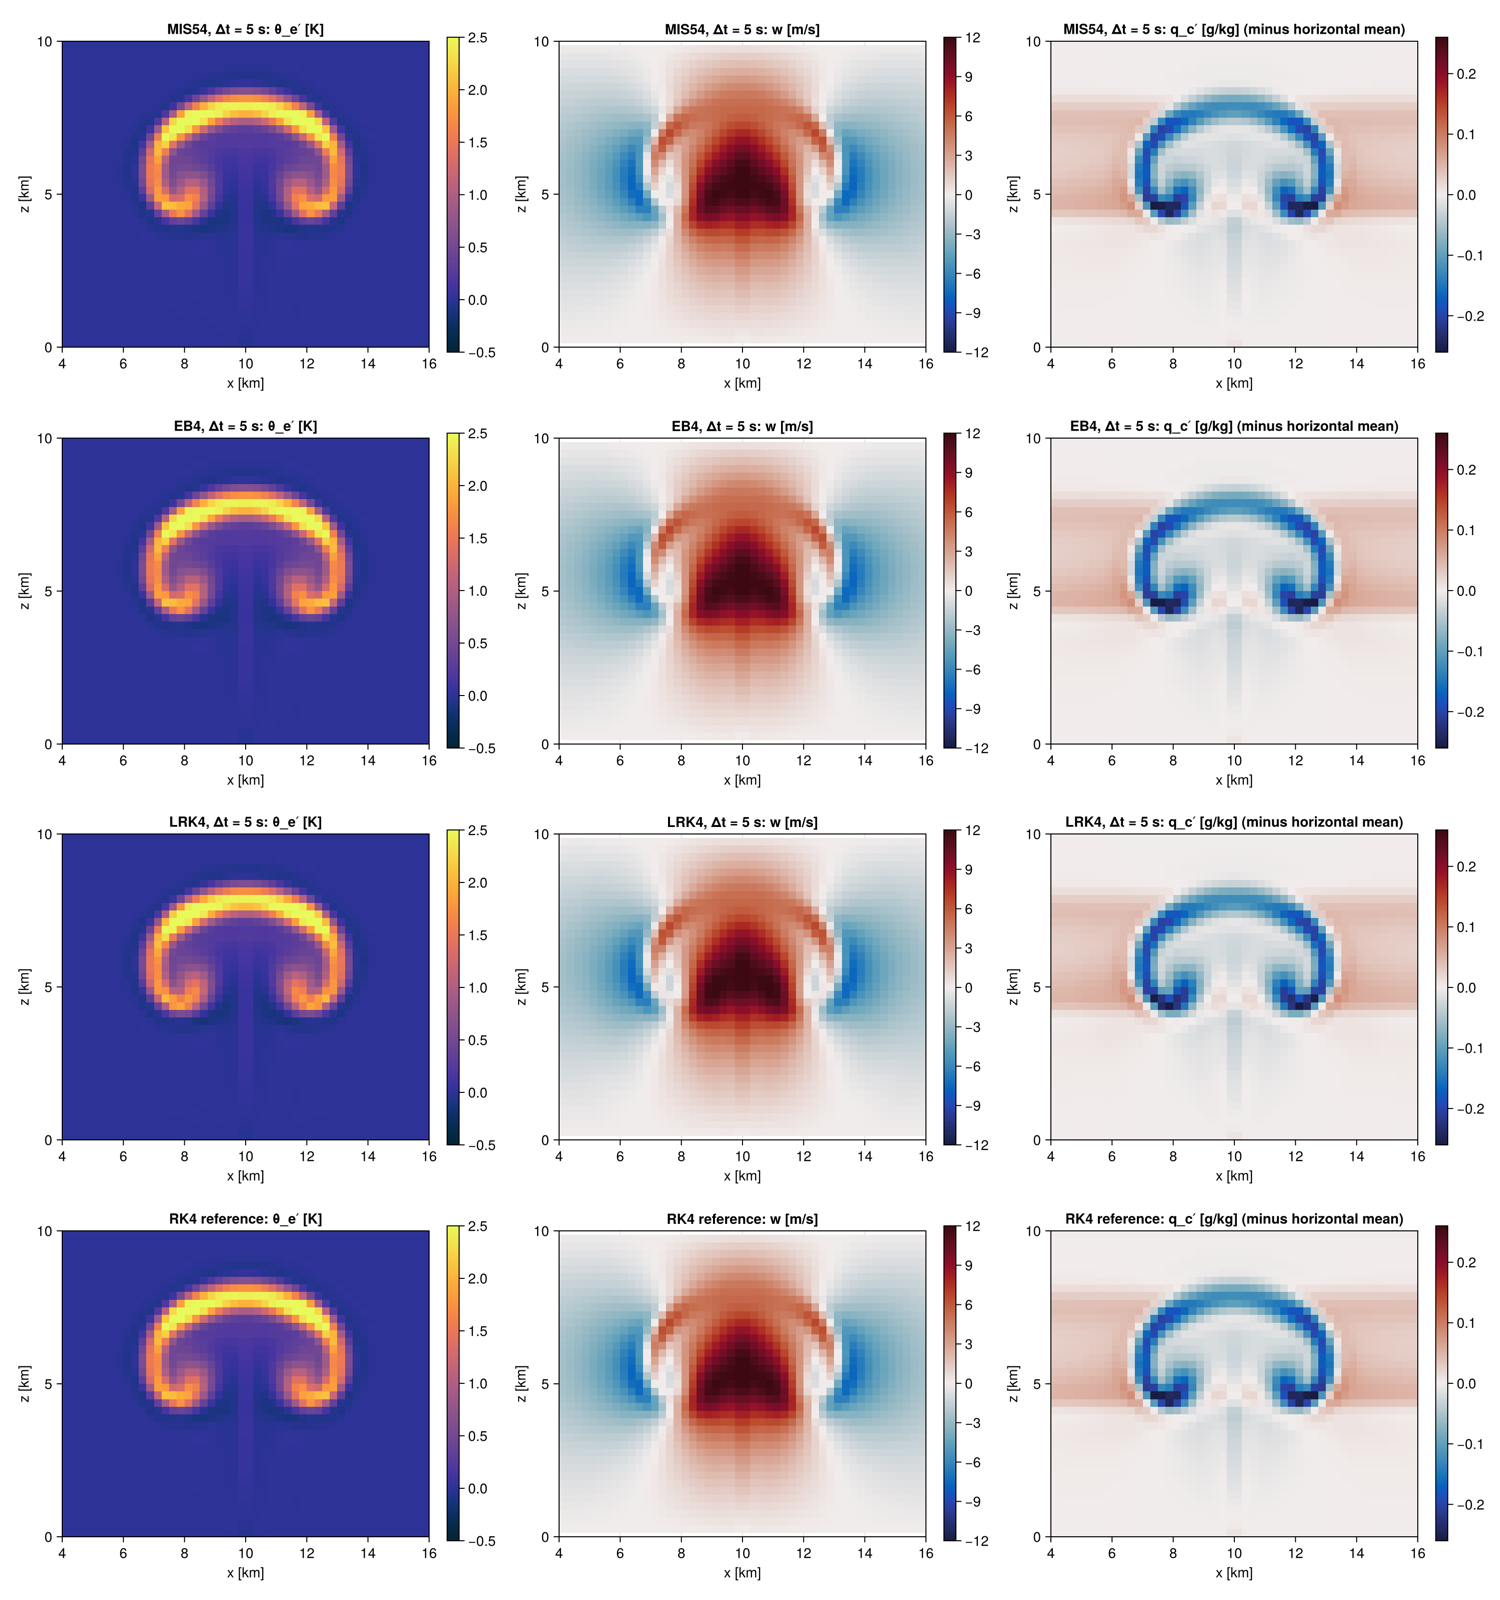
\includegraphics[width=0.92\textwidth]{bubble_thetarho_pi.png}
\caption{Moist bubble at 1000\,s, $X=\rho\theta_\rho$, $\pv=\pi$, $\tau_{\rm fac}=4$, Verlet EI with
$\varepsilon=0.1$, $\dt=5$\,s ($n_{\rm sub}=10$): $\theta_e'$, $w$ and $q_c'$ (deviation from the horizontal mean)
for MIS54, EB4, LRK4 and the RK4 reference. In the saturated environment the bubble carries less
condensate than its surroundings ($q_c'<0$).}\label{fig:bubble}
\end{figure}
\begin{figure}[htbp]\centering
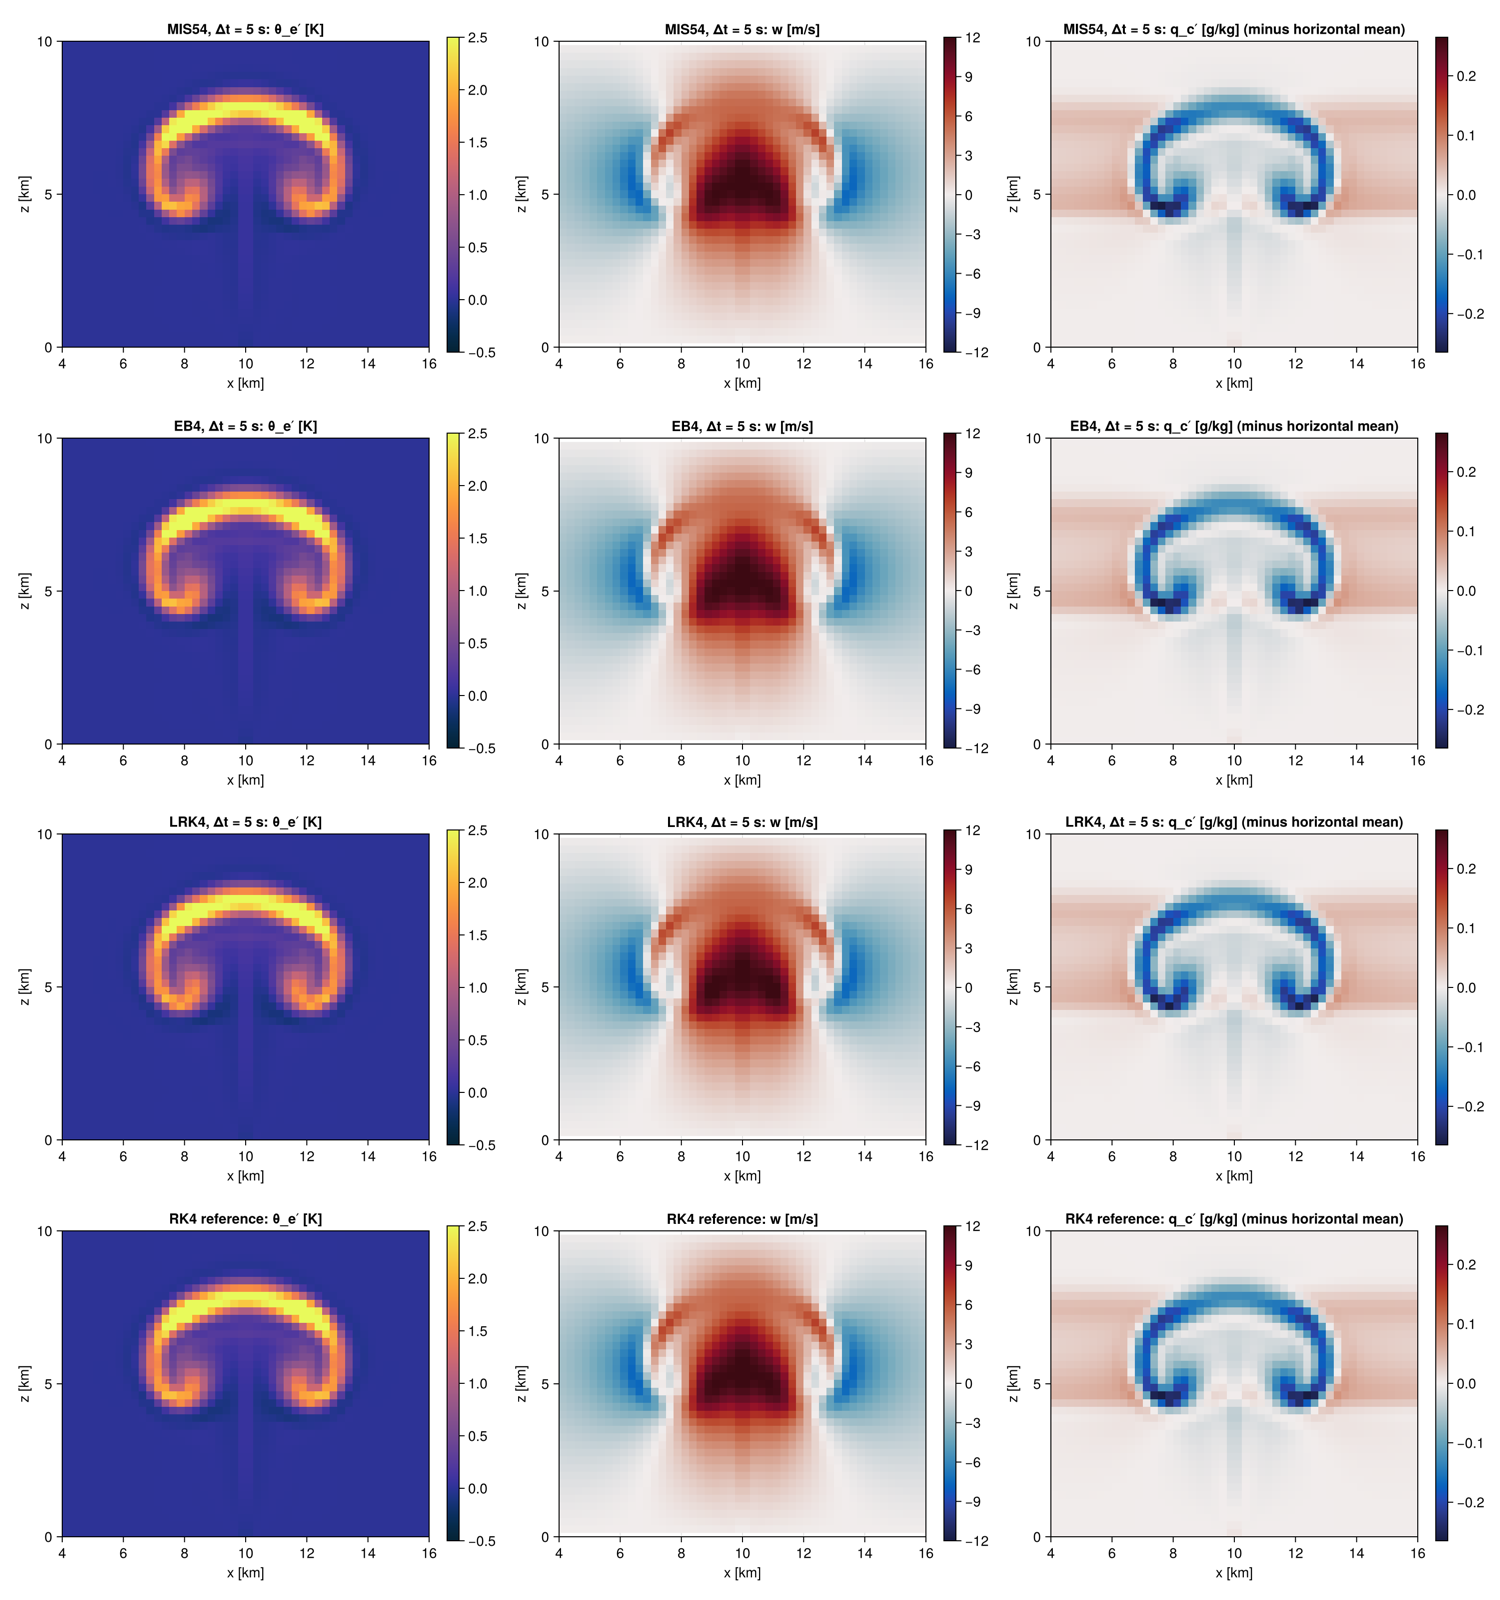
\includegraphics[width=0.92\textwidth]{bubble_energy_p.png}
\caption{As Figure~\ref{fig:bubble}, with the internal energy $X=\rho e$ and the pressure $\pv=p$.}\label{fig:bubble_e}
\end{figure}

\paragraph{Short relaxation and the limit of the explicit phase change.} In the Verlet EI step the phase
change is part of \code{:hthermo} and is applied once per small step with the total weight $h$ (split
into $(1-\beta)h$ and $\beta h$, combined between steps). An explicit relaxation step
$y\leftarrow y-(h/\tau)y$ needs $h/\tau\le2$, so EI needs $\tau\gtrsim\dtau/2$, i.e.\ $\tau_{\rm fac}\gtrsim0.45$ at
$\dtau\approx\dtau_{\rm ac}$; the code default $\tau_{\rm fac}=0.25$ is below this limit. At
$\tau_{\rm fac}=0.5$ ($\tau=0.28$\,s, $h=0.5$\,s, $h/\tau=1.8$), maximum error of $\theta_e'$ [mK] at
$\dt=2/5/10$\,s (f: failed):
\begin{center}\small
\begin{tabular}{llccc}\toprule
$X$ & $\pv$ & MIS54 & EB4 & LRK4\\\midrule
$\rho\theta_\rho$ & $\pi$ & 2.6 / $3\cdot10^4$ / f & 3.7/3.6/6.0 & 162/f/f\\
$\rho\theta_\rho$ & $p$ & 2.7 / $3\cdot10^4$ / f & 3.8/3.7/3.0 & 165/f/f\\
$\rho e$ & $\pi$ & 3.1 / $5\cdot10^3$ / f & 4.5/4.4/6.9 & 170/f/f\\
$\rho e$ & $p$ & 3.1 / $5\cdot10^3$ / f & 4.6/4.5/3.5 & 172/f/f\\\bottomrule
\end{tabular}
\end{center}
(RK4: $\max|w|=13.26$\,m/s for $\rho\theta_\rho$, 13.30 for $\rho e$.) The small step $h$ is the same for all
$\dt$ ($\dt/n_{\rm sub}=0.50$--0.53\,s), so the failure is not the fast step alone. ETD (EB4) stays at
3--7\,mK up to $\dt=10$\,s; MIS54 and LRK4 fail from $\dt=5$\,s. In EB4 every stage starts from $q^n$ and the
fast coefficients are those of $q^n$; in MIS the stage starts from $q^n+\sum\alpha_{ij}\Delta Y_j$ and the
coefficients are combinations with negative weights $w_{ij}$, and in Lawson the slow remainder is added
in jumps $\dt\,a_{ij}\tilde S$: both put the fast loop into states further from phase equilibrium, where
the explicit relaxation at $h/\tau\approx2$ has no margin. This is an observation, not an analysis. With the
energy variable MIS54 degrades more slowly ($5\cdot10^3$ instead of $3\cdot10^4$\,mK at 5\,s), consistent with
$Q_X=0$: the phase change does not feed back into $X$ directly. \emph{Recommendation for EI}: $\tau_{\rm fac}\ge1$
(resolved relaxation; at $\tau_{\rm fac}=4$ all runs above are stable up to $\dt=10$\,s), or a linearly implicit
relaxation in the small step (open).

%======================================================================
\section{Moist flow over a hill}\label{sec:hill}
Hydrostatic mountain wave over an Agnesi hill (Gallus and Klemp 2000): $h_0=400$\,m, $a=10$\,km,
$U=10$\,m/s, $N=0.01$\,s$^{-1}$ (dry $\theta$, $\theta_0=288$\,K), relative humidity $RH_0=0.85$ below 7\,km,
decreasing to 20\,\% at 9\,km; periodic channel 400\,km, top 12\,km, Rayleigh damping of $W$ above
8\,km; terrain-following grid $200\times48$ ($\Delta x=2$\,km, $\Delta\eta=250$\,m), explicit metric term
($c_s\dtau|z_x|/\Delta z\approx0.2$); every column in discrete hydrostatic balance with its own $J\Delta\eta$;
impulsive start; $T=6$\,h. $\dt=30$\,s, $n_{\rm sub}=7$ ($\dtau=4.29$\,s, vertical acoustic Courant number
$c_s\dtau/\Delta z\approx6$); Verlet EI with $\varepsilon=0.1$; $\tau_{\rm fac}=0.5$ ($\tau=2.2$\,s).
\begin{center}\code{RH0=0.85 TAUFAC=0.5 THVAR=thetarho|energy PVAR=pi|p METHOD=MIS54|EB4|LRK4 FAST=ei OFFCENTER=0.1\\
julia --project=examples examples/frozen\_moist\_hill.jl}\end{center}

\paragraph{Relaxation time.} With EI the default $\tau_{\rm fac}=0.25$ of \code{docs/exner} ($h/\tau=3.8$) is unstable
(the run breaks down after 40--50\,min) and $\tau_{\rm fac}=0.3$ ($h/\tau=3.2$) gives a wrong
solution ($\max|w|=16$\,m/s after 1\,h); $\tau_{\rm fac}\ge0.4$ is correct, and between 0.4 and 2 the solution
after 1.5\,h changes by less than 2\,\% in $\max|w|$ and 8\,\% in $\max q_c$. The limit $h/\tau\lesssim2.5$ is that of
Section~\ref{sec:bubble}. The runs use $\tau_{\rm fac}=0.5$ ($h/\tau=1.9$).

\paragraph{Results after 6\,h.} No run is unstable; mass and total water are conserved to
$\le2\cdot10^{-14}$. Cloud ($q_c>10^{-5}$) in all moist runs: a shallow cap cloud over the crest and a
wave cloud at 5.5--7.8\,km above and just downstream of the hill (maximum at $x-x_m=1$--3\,km,
$z=6.55$\,km), plus a small cloud at 4.7\,km, 25\,km downstream; the dry run has
$\max|w|=0.71$\,m/s.
\begin{center}\small
\begin{tabular}{llllccc}\toprule
$X$ & $\pv$ & method & fast step, $\dt$ & $\max|w|$ [m/s] & $\max q_c$ [g/kg] & time [s]\\\midrule
$\rho\theta_\rho$ & $\pi$ & MIS54 & EI $\varepsilon=0.1$, 30\,s & 0.980 & 0.168 & 400\\
$\rho\theta_\rho$ & $p$ & MIS54 & EI $\varepsilon=0.1$, 30\,s & 0.967 & 0.165 & 378\\
$\rho e$ & $\pi$ & MIS54 & EI $\varepsilon=0.1$, 30\,s & 0.933 & 0.165 & 370\\
$\rho e$ & $p$ & MIS54 & EI $\varepsilon=0.1$, 30\,s & 0.920 & 0.162 & 339\\
$\rho\theta_\rho$ & $\pi$ & EB4 & EI $\varepsilon=0.1$, 30\,s & 0.980 & 0.168 & 552\\
$\rho\theta_\rho$ & $p$ & EB4 & EI $\varepsilon=0.1$, 30\,s & 0.968 & 0.165 & 534\\
$\rho\theta_\rho$ & $\pi$ & LRK4 & EI $\varepsilon=0.1$, 30\,s & 1.122 & 0.178 & 490\\
$\rho\theta_\rho$ & $p$ & LRK4 & EI $\varepsilon=0.1$, 30\,s & 0.934 & 0.177 & 471\\
$\rho\theta_\rho$ & $p$ & MIS54 & EI $\varepsilon=0.1$, 60\,s & 0.925 & 0.160 & 293\\
$\rho e$ & $p$ & MIS54 & EI $\varepsilon=0.1$, 60\,s & 0.882 & 0.158 & 265\\
$\rho\theta_\rho$ & $\pi$ & MIS54 & EI $\varepsilon=0$, 30\,s & 0.974 & 0.167 & 388\\
\midrule
dry & $\pi$ & MIS54 & EI $\varepsilon=0.1$, 30\,s & 0.714 & -- & 399\\\bottomrule
\end{tabular}
\end{center}
(Times: serial runs, 13 runs in parallel on 16 cores; only the ratios are meaningful.) There is no
reference solution; the differences between the runs are given as maximum differences of the fields
at 6\,h ($|x-x_m|\le60$\,km) relative to $\max|w|$ and $\max q_c$:
\begin{center}\small
\begin{tabular}{lccc}\toprule
comparison & $\Delta w/\max|w|$ & $\Delta q_c/\max q_c$ & $\max|\Delta RH|$\\\midrule
MIS54 / EB4 & 0.5\,\% & 0.7\,\% & 0.001\\
$\pi$ / $p$ ($\rho\theta_\rho$) & 1.6\,\% & 2.5\,\% & 0.005\\
$\dt=30$ / 60\,s ($\rho\theta_\rho$, $p$) & 5.6\,\% & 21\,\% & 0.016\\
$\dt=30$ / 60\,s ($\rho e$, $p$) & 5.6\,\% & 20\,\% & 0.014\\
$\rho\theta_\rho$ / $\rho e$ ($\pi$) & 9.1\,\% & 6.6\,\% & 0.015\\
$\rho\theta_\rho,\pi$ / $\rho e,p$ & 9.4\,\% & 7.5\,\% & 0.017\\
EI $\varepsilon=0.1$ / EI $\varepsilon=0$ & 21\,\% & 4.4\,\% & 0.004\\
MIS54 / LRK4 & 32\,\% & 18\,\% & 0.068\\\bottomrule
\end{tabular}
\end{center}
\begin{itemize}
\item \emph{MIS54 and EB4} agree to 0.5\,\% in $w$ (Figure~\ref{fig:hill_eb4}); EB4 costs 40\,\% more (two fast
integrations of the stages from $q^n$ and the remainder evaluations).
\item \emph{LRK4} carries a spurious wave train of $\approx10$\,km horizontal wavelength through the whole
channel, deepest above 4\,km, amplitude 0.3\,m/s (Figure~\ref{fig:hill_lrk4}); the cloud is almost unchanged.
It is not in the dry part of the mountain wave of MIS54 and EB4 and is attributed to the jumps
$\dt\,a_{ij}\tilde S$ of the Lawson step (not analysed).
\item \emph{Thermodynamic variable}: $\rho\theta_\rho$ and $\rho e$ give the same wave and the same clouds
(Figure~\ref{fig:hill_thvar}); the difference, 9\,\% in $w$, is a short wave pattern in the lee (10--20\,km
downstream, all heights), of the size of the difference of the two spatial discretizations seen in the
bubble. The pressure variable matters less (1.6\,\%).
\item \emph{Large step}: $\dt=60$\,s ($n_{\rm sub}=14$) is stable for both thermodynamic variables and changes
the cloud water by 20\,\% (Figure~\ref{fig:hill_dt60}): the cloud edges are sharp and the advective time scale
of the cloud ($\Delta x/U=200$\,s) is only three to four large steps.
\item \emph{Off-centring}: without it (EI, $\varepsilon=0$) the run is stable, but a deep mode with a horizontal
wavelength of about 80\,km and amplitude 0.2\,m/s remains from the impulsive start (Figure~\ref{fig:hill_ei0});
$\varepsilon=0.1$ removes it. Near the hill and in the cloud the two agree within 4\,\% ($q_c$).
\end{itemize}

\begin{figure}[htbp]\centering
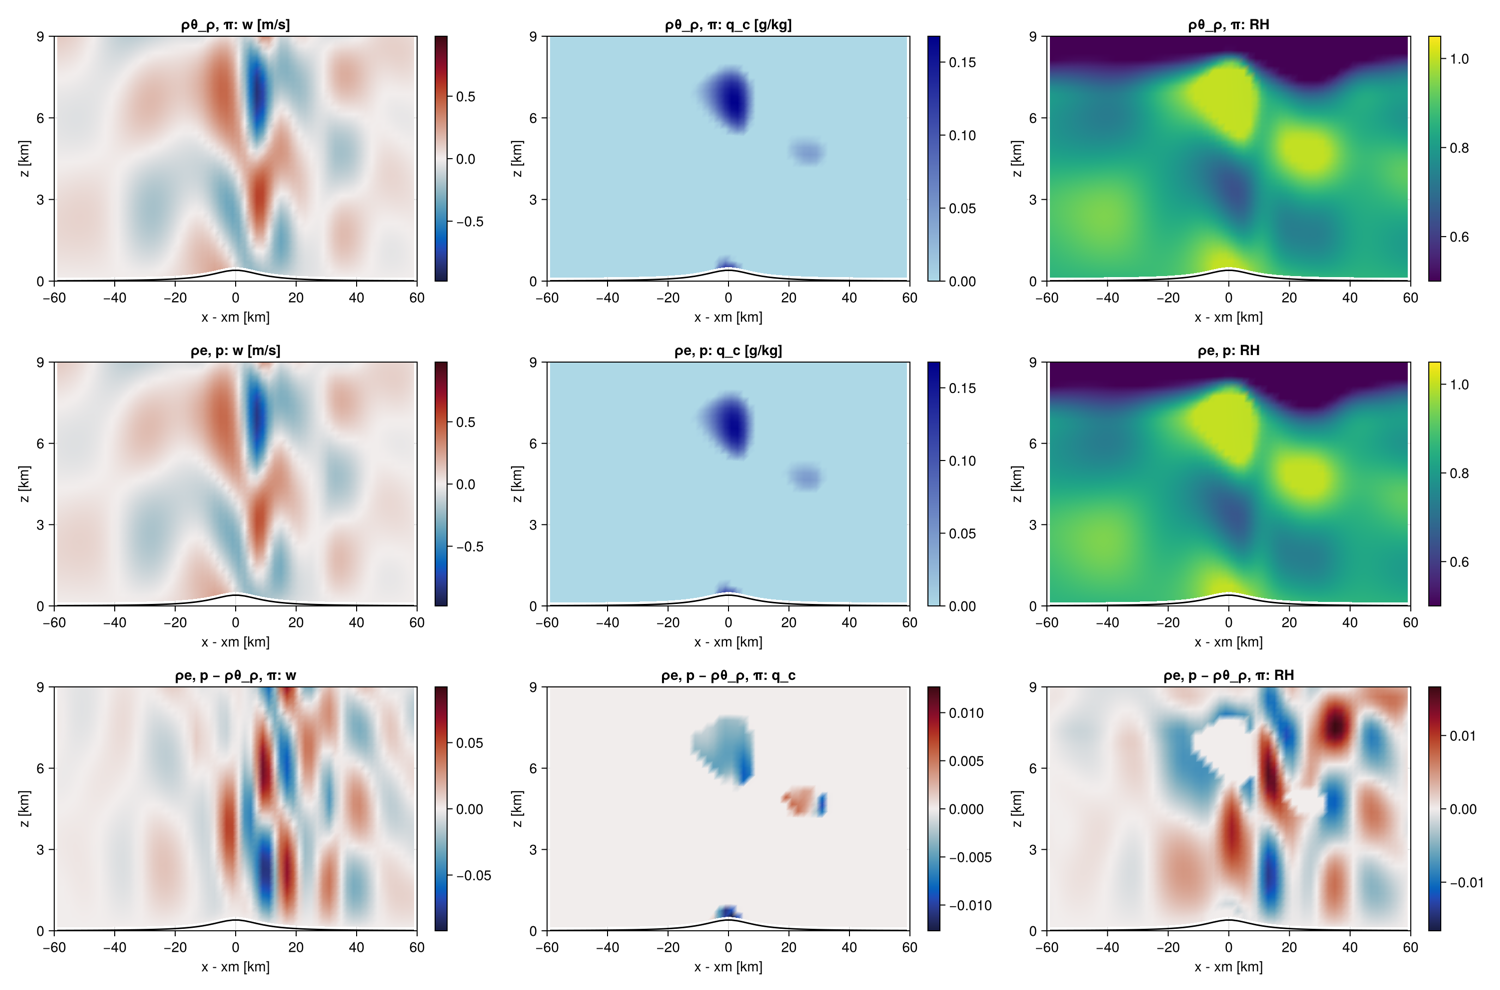
\includegraphics[width=\textwidth]{hill_thvar.png}
\caption{Moist mountain wave after 6\,h, MIS54, EI $\varepsilon=0.1$, $\dt=30$\,s: $w$, $q_c$ and RH with $X=\rho\theta_\rho$,
$\pv=\pi$ (top) and $X=\rho e$, $\pv=p$ (middle), and their difference (bottom).}\label{fig:hill_thvar}
\end{figure}
\begin{figure}[htbp]\centering
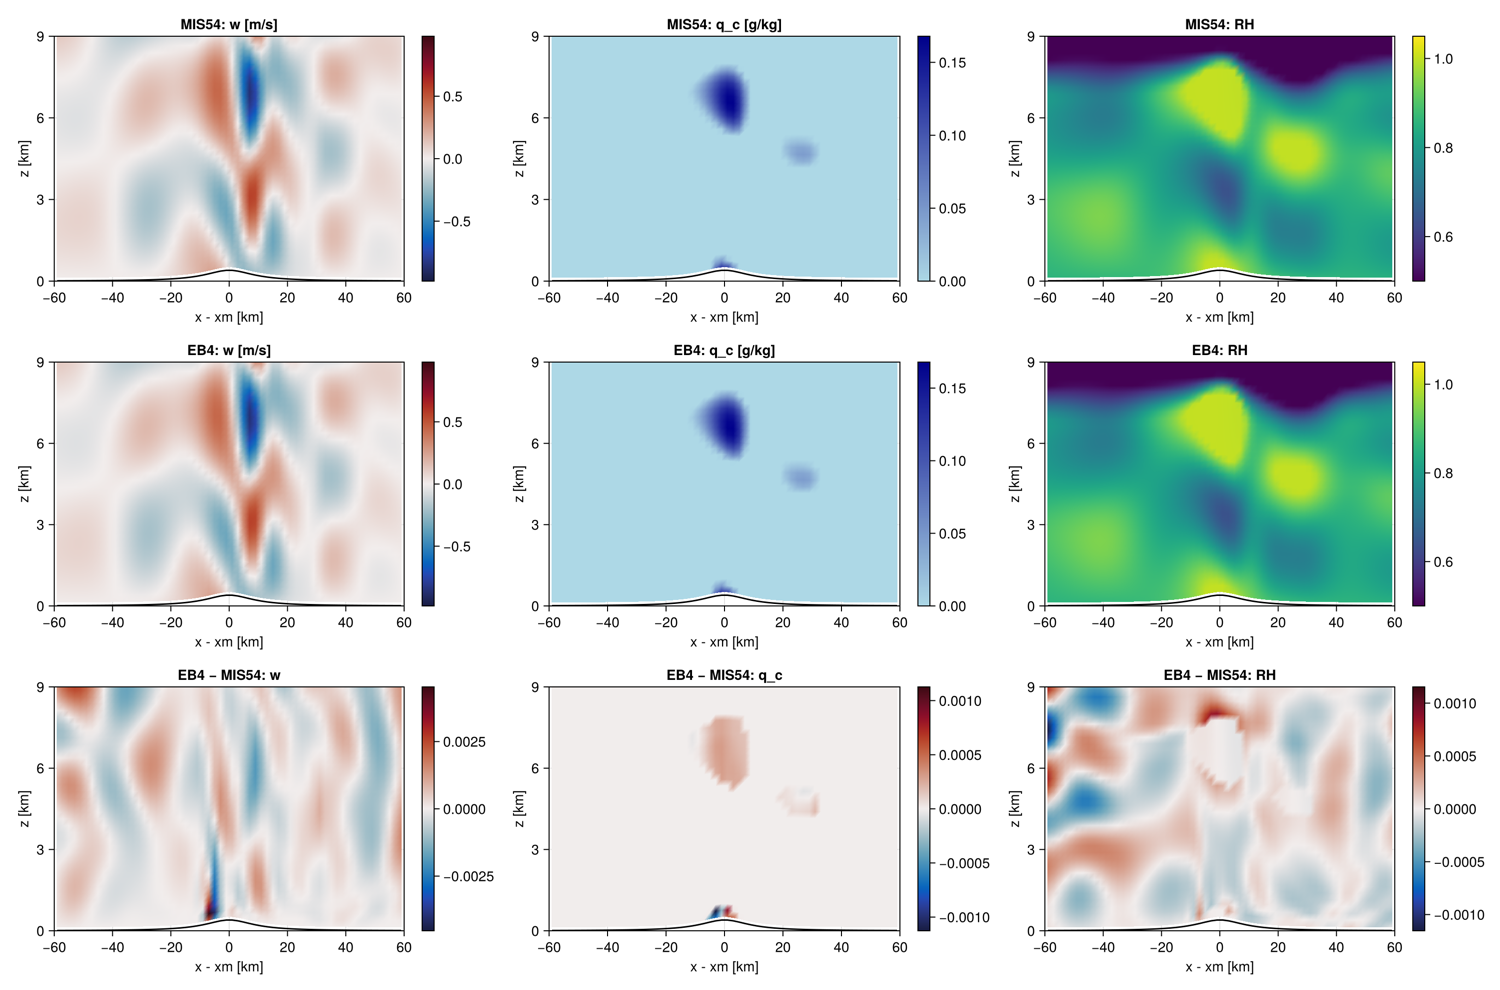
\includegraphics[width=\textwidth]{hill_eb4.png}
\caption{As Figure~\ref{fig:hill_thvar}, $X=\rho\theta_\rho$, $\pv=\pi$: MIS54 (top) and the ETD method EB4 (middle).}\label{fig:hill_eb4}
\end{figure}
\begin{figure}[htbp]\centering
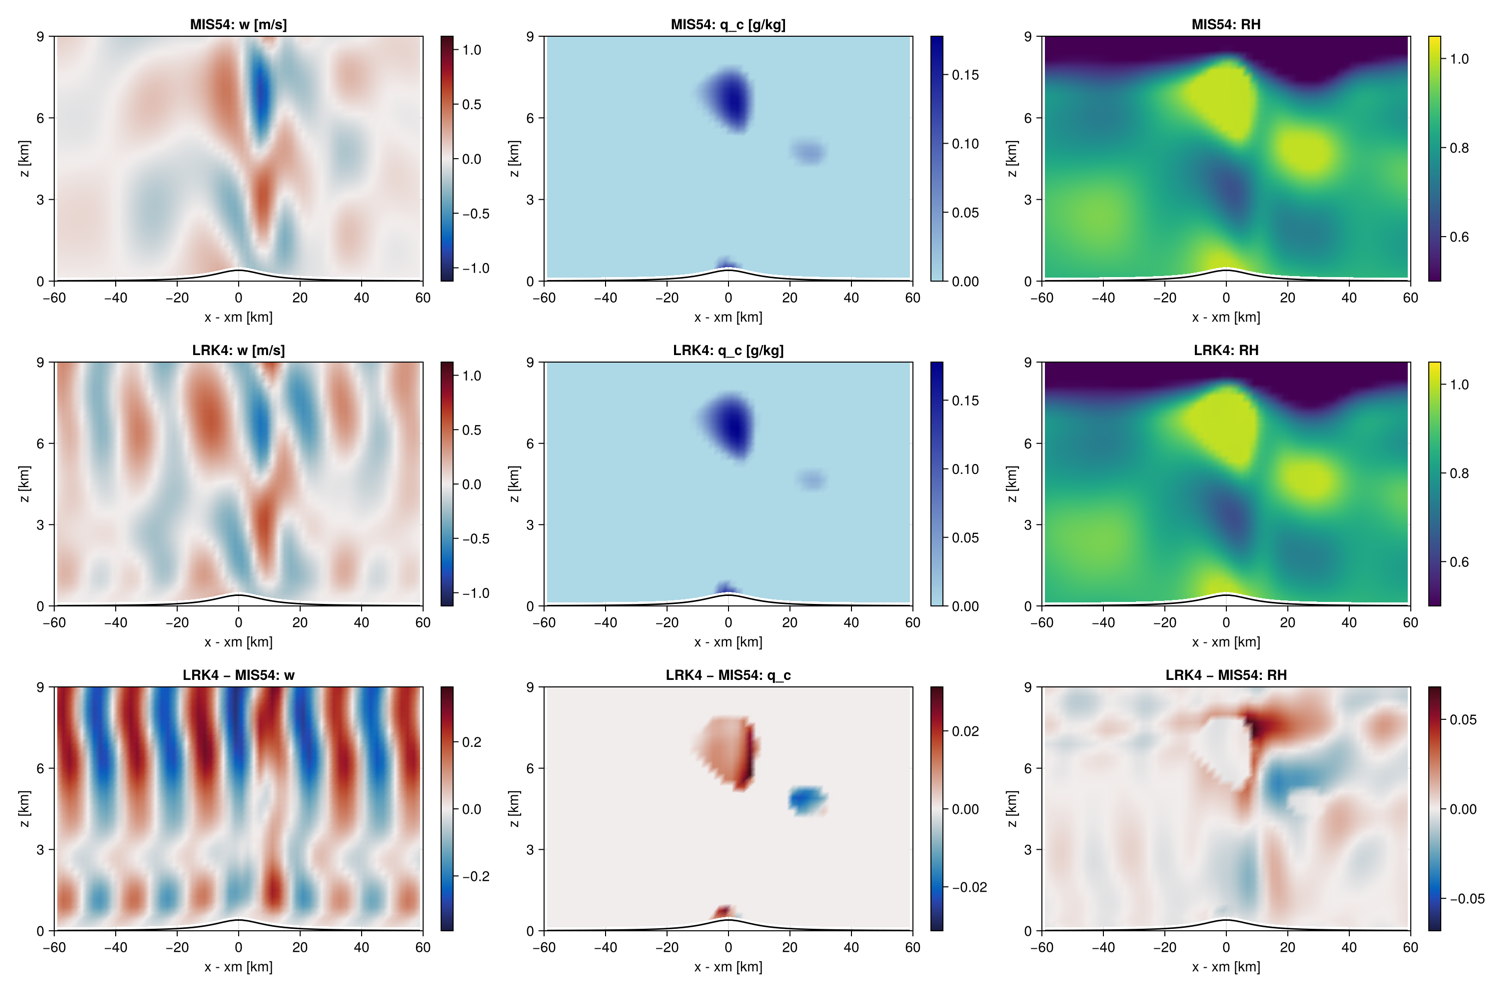
\includegraphics[width=\textwidth]{hill_lrk4.png}
\caption{MIS54 (top) and the Lawson method LRK4 (middle): spurious wave train of LRK4.}\label{fig:hill_lrk4}
\end{figure}
\begin{figure}[htbp]\centering
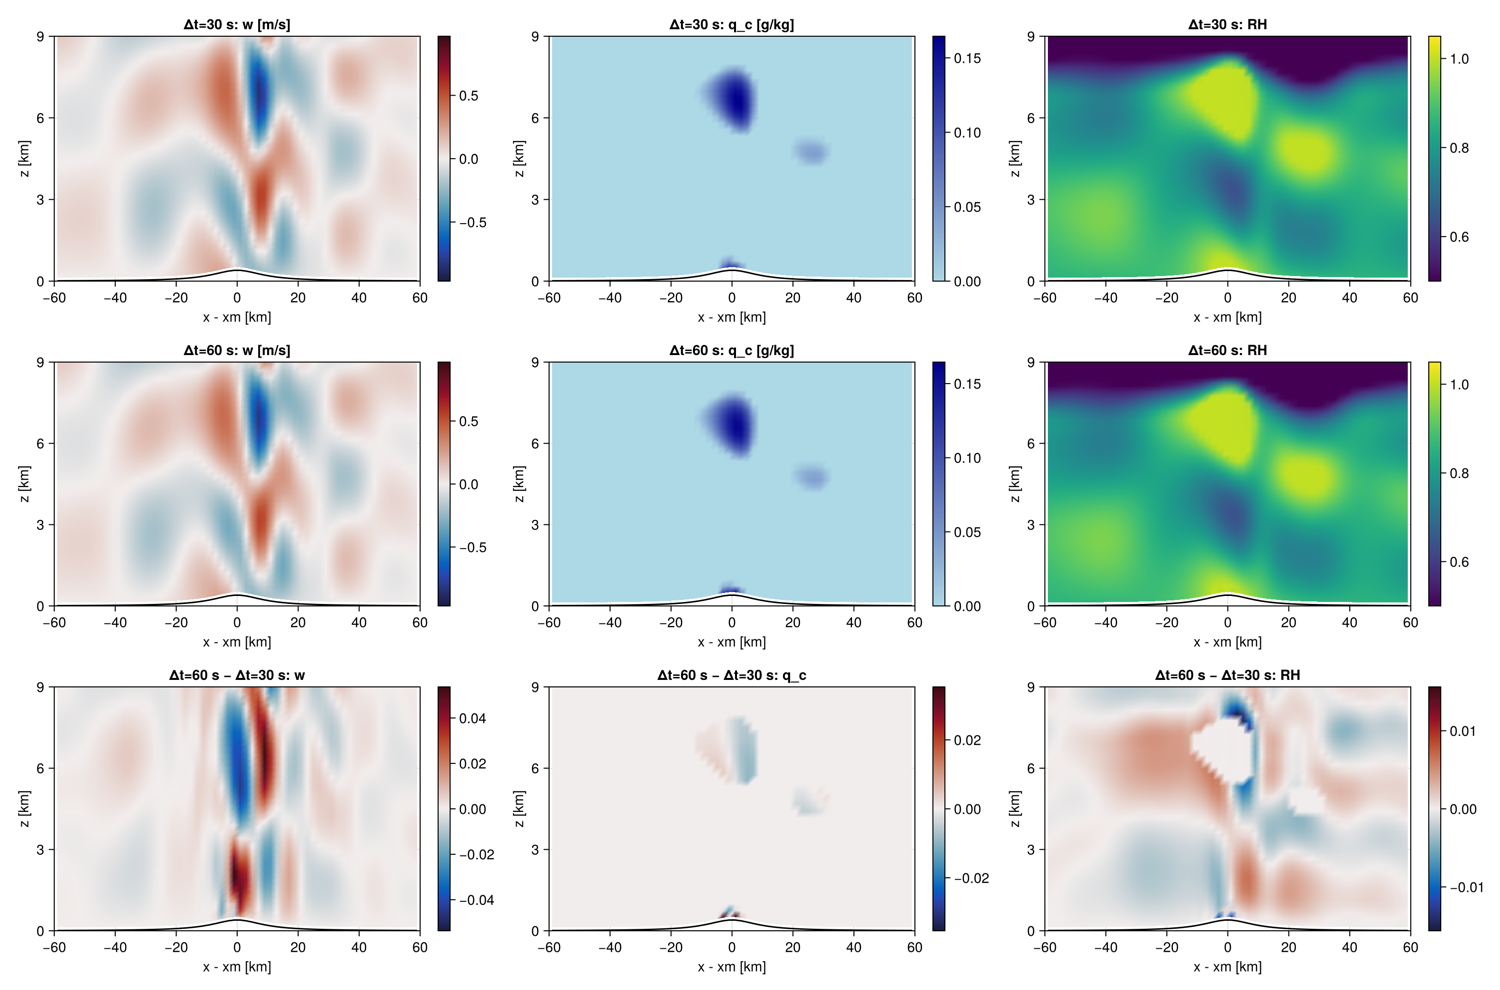
\includegraphics[width=\textwidth]{hill_dt60.png}
\caption{$X=\rho\theta_\rho$, $\pv=p$, MIS54: $\dt=30$\,s ($n_{\rm sub}=7$, top) and $\dt=60$\,s ($n_{\rm sub}=14$, middle).}\label{fig:hill_dt60}
\end{figure}
\begin{figure}[htbp]\centering
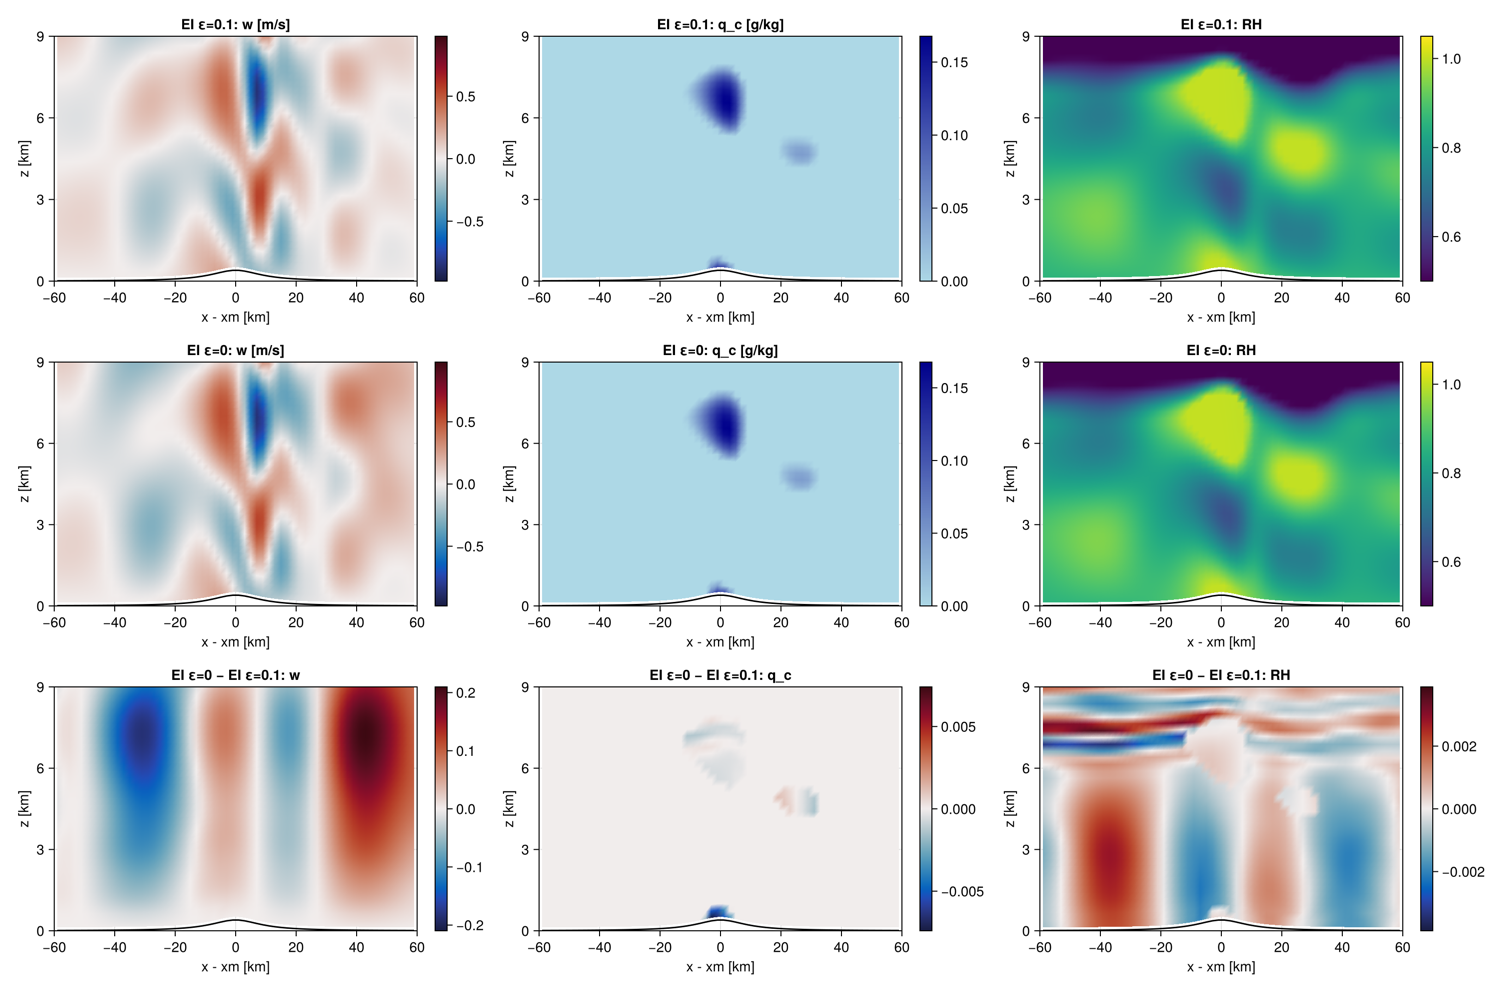
\includegraphics[width=\textwidth]{hill_ei0.png}
\caption{Verlet EI with $\varepsilon=0.1$ (top) and without off-centring (middle): deep mode of the impulsive start.}\label{fig:hill_ei0}
\end{figure}

%======================================================================
\section{Conclusions and open points}
\begin{enumerate}
\item With the pressure (or Exner pressure) as an additional variable the fast acoustic--gravity
system is closed in $(\rho,\pv,U,W)$; the thermodynamic variable and the two moisture variables are
transported by the live mass flux with frozen face values and follow from the column solve by back
substitution. One tridiagonal system per column covers both thermodynamic variables, both pressure
variables, dry and moist; the small step is neutral up to vertical Courant numbers far above one.
\item $X=\rho\theta_\rho$ and $X=\rho e$ are equally accurate and stable in time. $\rho e$ needs no latent-heating
source; $\rho\theta_\rho$ is a flux-form variable. The two spatial discretizations differ by 5--9\,\%; a
resolution study is needed to say which is closer to the converged solution.
\item Verlet EI as the fast integrator: errors of 1--9\,mK in $\theta_e'$ in the bubble with MIS54 and EB4, one
column solve and one evaluation of each part per small step; $\varepsilon=0.1$ is needed against the modes of
the impulsive start on the hill.
\item MIS54 and ETD (EB4) agree; ETD is more robust near the stability limit of the explicit phase
change, MIS cheaper. Lawson (LRK4) is not competitive: 50--300 times larger errors in the bubble and a
spurious wave train on the hill.
\item The explicit relaxation needs $\dtau/\tau\lesssim2$ with EI: $\tau_{\rm fac}\ge0.5$, better
$\ge1$. A linearly implicit relaxation in the small step (the phase change as part of the column, or a
pointwise implicit step after the horizontal part) would remove the limit and is the next step.
\item Open: steep terrain with the implicit metric term (\code{FV\_METRIC\_IMPLICIT}), moist WRF
fast step, total energy as $X$, limiter for the moisture reconstruction, rain.
\end{enumerate}

\end{document}
